\chapter{Model} % is the methodology
\label{ch:model-methodology}


    \section{Application Model}
    \label{sec:application-model}

    % An application model in research refers to a conceptual or theoretical framework that describes the structure, behavior, and interactions of a software application. It is a high-level representation of the system that captures its essential features, without getting into the details of its implementation.

    % Application models are often used in research to analyze and design software applications, to identify potential problems or limitations, and to evaluate different approaches to solving them. They can be used to describe different aspects of the application, such as its functionality, performance, usability, and security.

    % One of the most common types of application models used in research is the software development life cycle (SDLC) model. The SDLC model describes the different stages involved in developing a software application, from the initial planning and requirements gathering to the final deployment and maintenance. Other application models used in research include the user-centered design (UCD) model, the agile development model, and the model-view-controller (MVC) model.

    % Overall, application models are an important tool in research for understanding and designing software applications, and they can help researchers to develop more effective and efficient systems.

    % TODO

    The application model structure is shown in figure \ref{fig:application-model}.
    The data pipeline is filled with task requests provided by users of the infrastructure.
    Section \ref{sec:data-pipeline-model} describes the data pipeline model and the components that are sent to the Deployment API.
    It is then sent to a server that consumes the data pipeline through a \emph{Deployment API}.
    Afterwards, the data pipeline is forwarded to the \emph{Preprocessing} component that prepares the data for further computations as described in section \ref{sec:data-preprocessing-techniques}.
    It is then sent to the adaptation component (see \ref{sec:resource-prediction-model}). The tasks with their adapted resource utilisation are then sent to the Scheduling component. 
    The tasks are scheduled and mapped onto available resources. 
    The mapped tasks are provided to the \emph{Orchestration} component which then deploys the tasks onto the resources defined in the schedule.



    % We model the applications as shown in figure \ref{fig:application-model}.
    % It consists of numerous components mentioned in previous sections and is the structural framework.
    % It receives tasks as a pipeline via a Deployment API that is sent to a \emph{Dependency Analysis} component.
    % After the dependency analysis, these tasks are sent to the \emph{Scheduling} component

    \begin{figure}
        \centering
        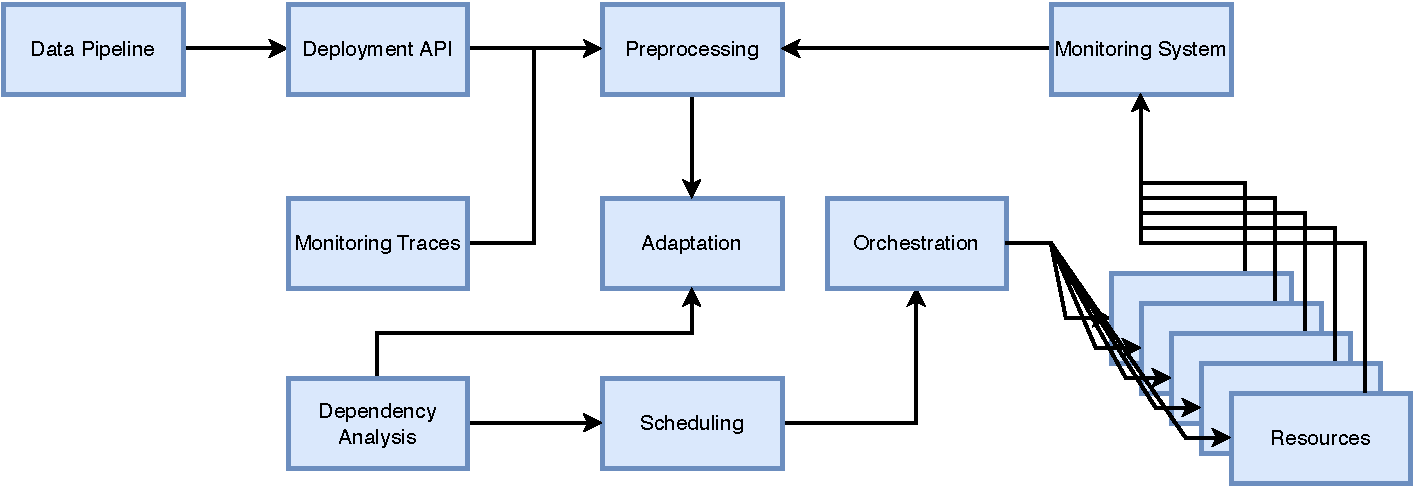
\includegraphics[width=0.8\textwidth]{figures/application_model.pdf}
        \caption{Application Model}
        \label{fig:application-model}
    \end{figure}
    \noindent
    The state of the resources is tracked by the monitoring system (see \ref{sec:monitoring-model}) and the states of all resources are collected with the Execution Event Detection (EED) component. In case of a rule violation is detected on a resource by the EED component, the tasks deployed on the resource are evaluated for possible adaptation.

    \section{Data Pipeline Model}
    \label{sec:data-pipeline-model}

        We model Big Data pipeline workflow received through the DEF-PIPE tool as $W = M, E, Q, M_{SOURCE}, M_{SINK}$, where $M$ is the set of Big Data pipeline tasks, $E$ denotes the Big Data pipelines, $Q$ is the data queue between the tasks, $M_{SOURCE}$ is the data producers (sources) and $M_{SINK}$ is the data consumers (sinks).


    % \section{Dependency Analysis}
    % \label{sec:dependency-analysis-model}

    \section{Resource Model}
    \label{sec:resource-model}

        We model the devices provided by the R-MARKET tool as a set of resources distributed over the computing continuum. 
        We define the set of resources as $R = {r_1, r_2, \dots, r_n}$, where $n = | R |$ denotes the total number of resources. 
        Thereafter, \CPUJUTIL shows a “non-idle” CPU of a resource $r_j$. 
        The \CPUJUTIL  is defined as \CPUJUTIL  = \CPUJBUSY  + \CPUJWAIT. \CPUJBUSY  and  \CPUJWAIT, respectively, show the amount of CPU that is “busy” with processing and “waiting” for other processes to be finished. In addition, we define the utilised memory as $\MEMJUTILMATH = \frac{\MEMJBUSYMATH}{\MEMJTOTALMATH}$.


    % In research, a resource model refers to a conceptual or theoretical framework that describes the resources required to complete a task or achieve a goal. It is a high-level representation of the resources that are available and needed in a particular context.

    % Resource models can be used in research to analyze and design systems or processes that require the allocation of resources, such as computer networks, transportation systems, and manufacturing plants. They can help researchers to understand the relationships between different resources, to identify potential bottlenecks or inefficiencies, and to evaluate different strategies for optimizing resource utilization.

    % One example of a resource model is a queueing model, which describes the behavior of queues or waiting lines in a system. Queueing models can be used to analyze the performance of different systems, such as call centers or traffic intersections, and to optimize their resource allocation and utilization.

    % Another example of a resource model is a network flow model, which describes the flow of resources through a network, such as a supply chain or a transportation system. Network flow models can be used to identify optimal routes or paths for resources, to allocate resources efficiently, and to optimize the performance of the system as a whole.

    % Overall, resource models are an important tool in research for understanding and designing systems that require the allocation and utilization of resources, and they can help researchers to develop more effective and efficient systems.

    \section{Network Model}
    \label{sec:network-model}

        We model the network channels between the computing resources as the round-trip latency LAT and network bandwidth BW between the resources $r_i$ and $r_j$.
        Afterwards, we denote the number of data bytes/packets sent and received to/from resources as: 
        $\DATASENTMATH = (\NETBYTESSENTMATH, \NETPACKETSSENTMATH)$ denotes the number of packets (in bytes) sent by the system to other resources.
        $\DATARecvMATH = (\NETBYTESRecvMATH, \NETPACKETSRecvMATH)$ denotes the number of packets (in bytes) received by the system from other resources.


        % In research, a network model refers to a conceptual or mathematical representation of a network, which is a collection of nodes and edges that are connected to each other in some way. A network model can be used to describe the structure, behaviour, and interactions of the network, and to analyze its properties and performance.

        % Network models are widely used in various fields of research, such as computer science, mathematics, engineering, and social sciences. They can be used to study a wide range of networked systems, such as communication networks, transportation networks, social networks, and biological networks.

        % One common type of network model is a graph model, which represents a network as a graph consisting of nodes and edges. Graph models can be used to analyze the connectivity of the network, identify important nodes or edges, and evaluate the resilience and robustness of the network to failures or attacks.

        % Another type of network model is a stochastic model, which incorporates randomness or uncertainty into the behaviour of the network. Stochastic models can be used to study the performance of the network under different conditions, such as varying traffic loads or node failures.

        % Overall, network models are an important tool in research for understanding and designing networked systems, and they can help researchers to develop more effective and efficient networks.

    \section{Monitoring Model}
    \label{sec:monitoring-model}

        The monitoring states \STATET that is sent at time step \TIMESTEPT from the resources to the Monitoring and Analysis component consisting of all monitoring metrics collected from the computing continuum. 
        Then, we define a capacity of a resource as MONrt, denoting the monitored data of resource r at time step \TIMESTEPT. 
        In this case, St is defined as $\STATETMATH = {MON_{r1}^\TIMESTEPTMATH, MON_{r2}^\TIMESTEPTMATH, \dots, MON_{rn}^\TIMESTEPTMATH}$ as the combination of monitored data of a resource $r_i$ at a time step \TIMESTEPT.

        
    \section{Resource Prediction Model}
    \label{sec:resource-prediction-model}

        The monitoring system on the computing continuum records the performance metrics, such as CPU, GPU, memory utilisation and network usage, along with the runtime execution of tasks. We train an LSTM-based machine learning model on the monitored and historical data. Then, the output is obtained from the LSTM prediction model. In the case that the difference between the prediction and monitored data is less than a threshold value (e.g., 0.1), we obtain the predicted under-utilized resources for task scheduling. Otherwise, we tune the training model parameters or add more historical data to improve the prediction accuracy.


        \begin{figure}
            \centering
            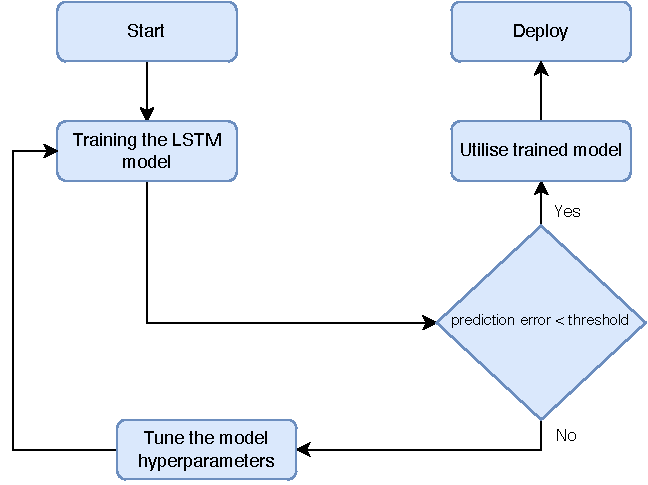
\includegraphics[width=0.9\textwidth]{figures/training_flowchart.pdf}
            \caption{Flow chart of resource prediction}
            \label{fig:flow-chart-of-resource-prediction}
        \end{figure}



        